\begin{figure}[t]
  \centering
  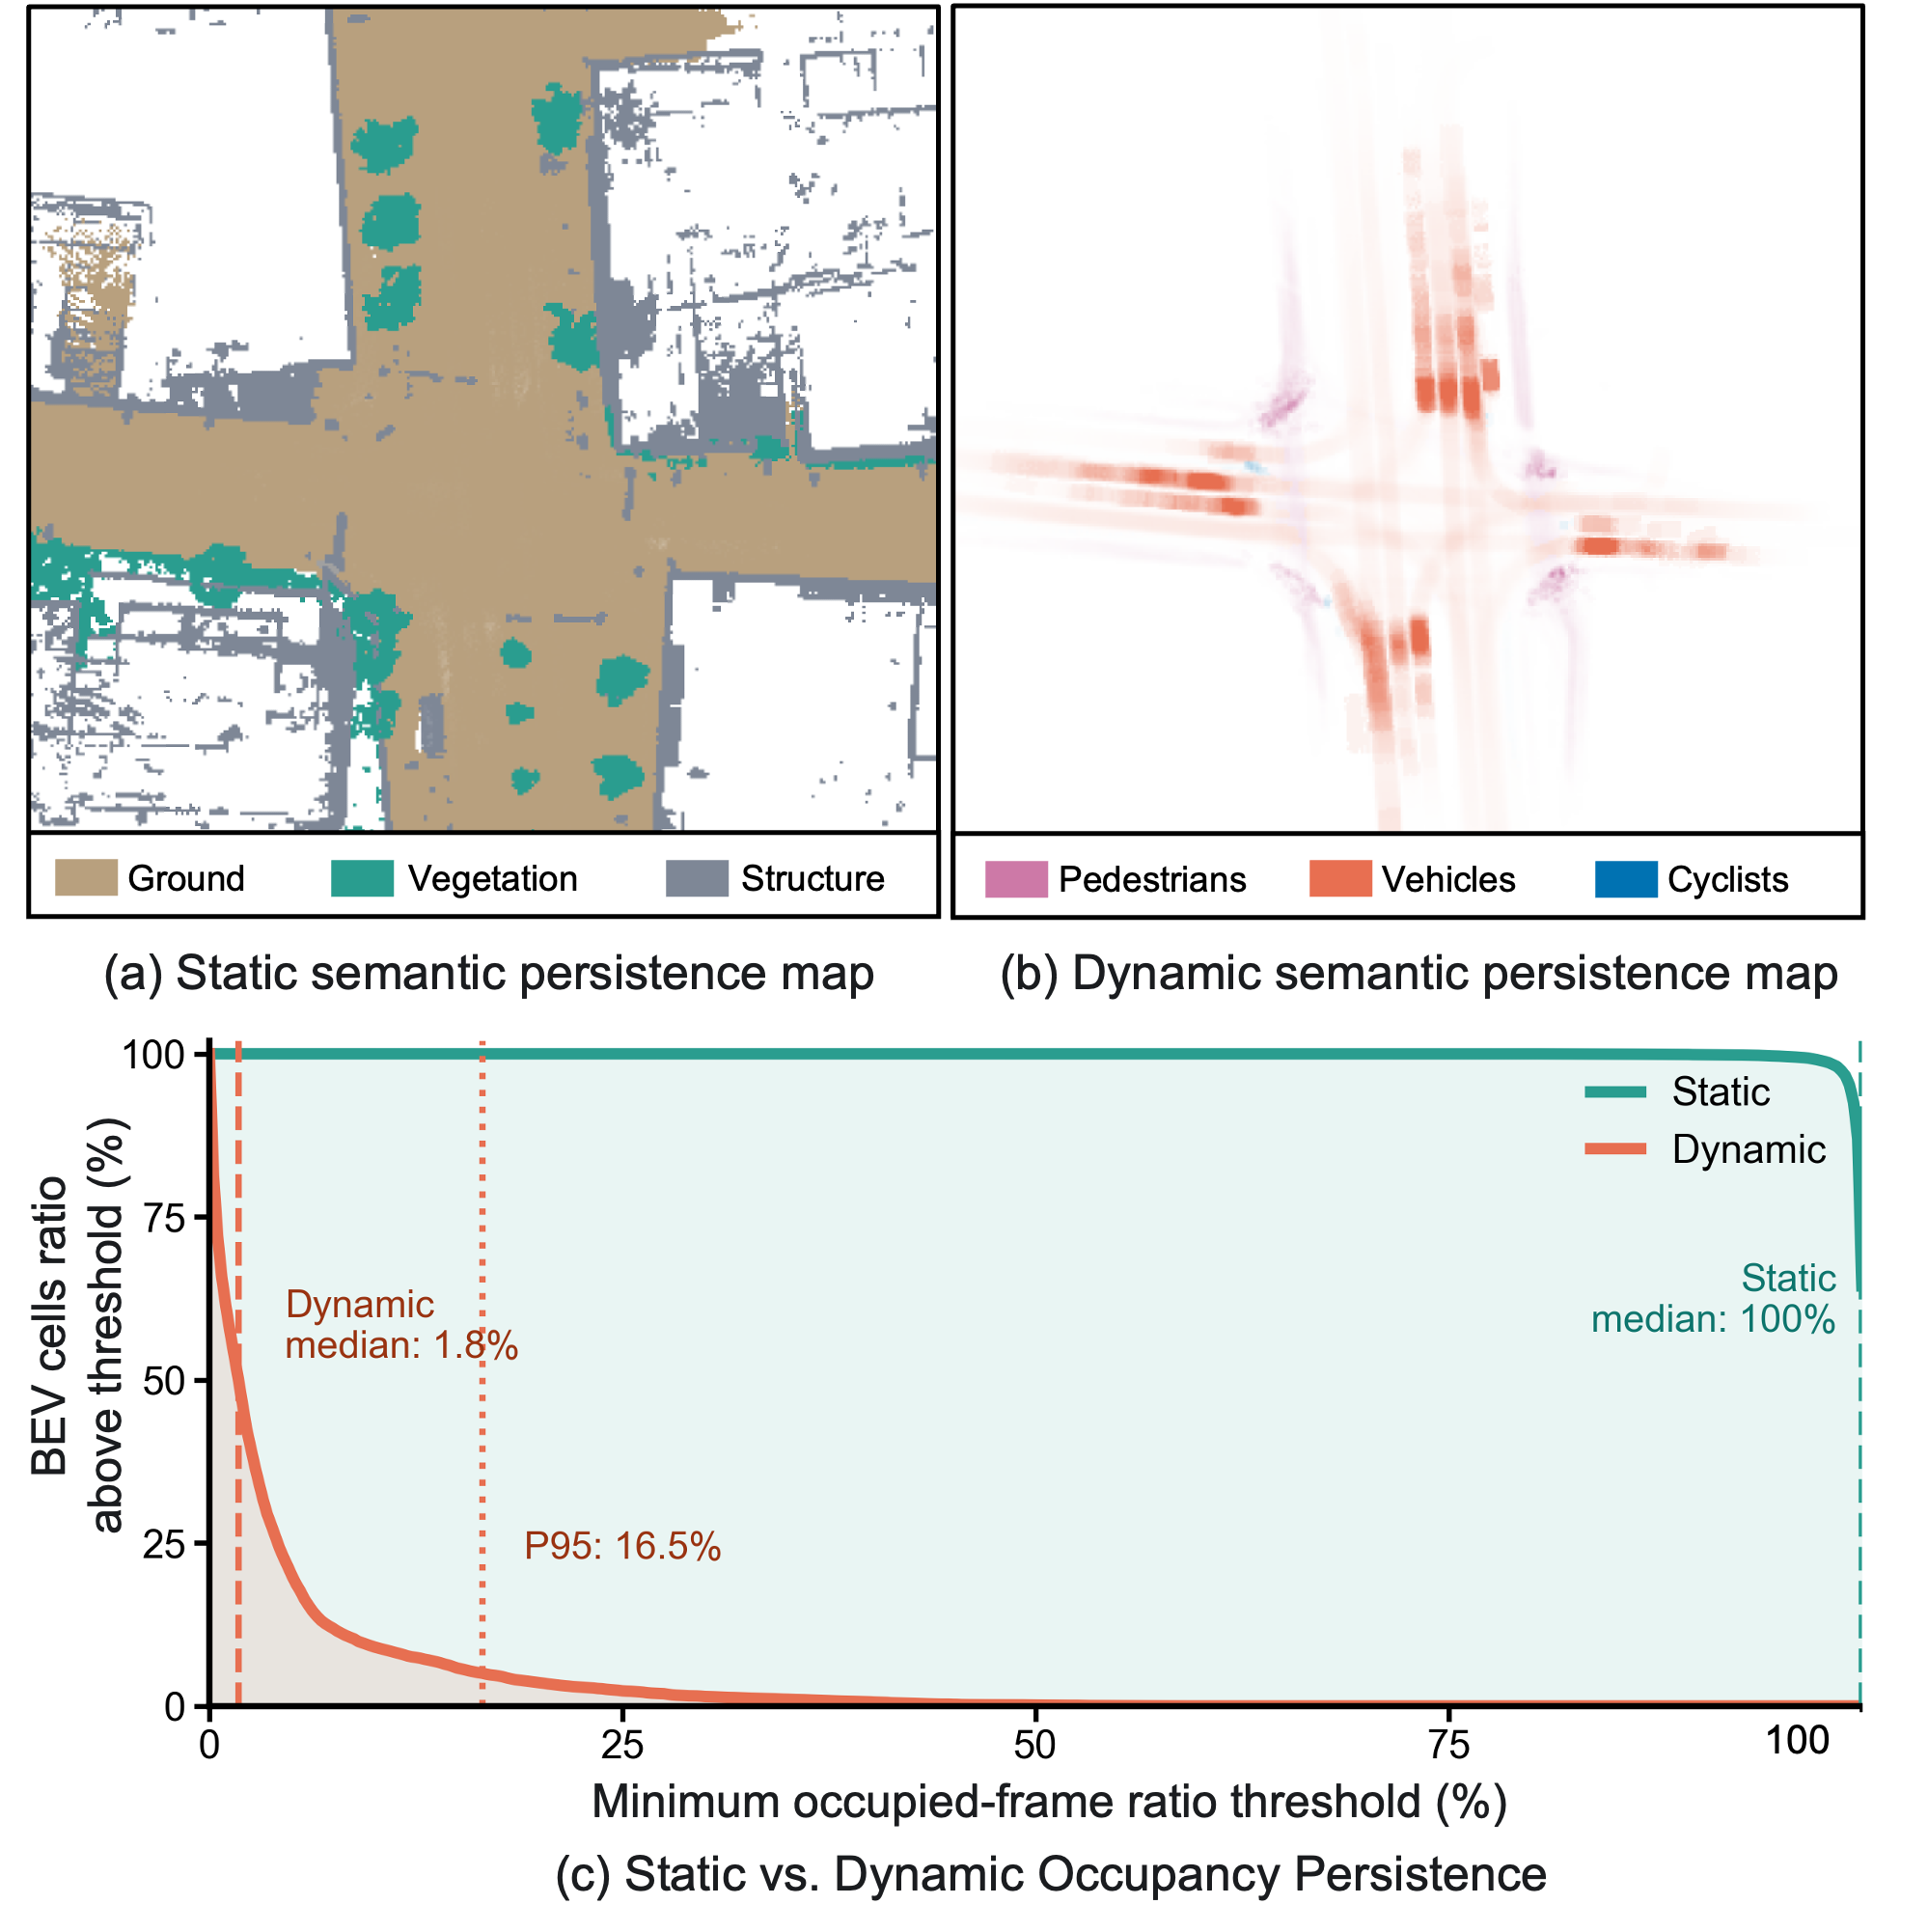
\includegraphics[width=\linewidth]{figures/fig06-temporal-statistics.png}
  \caption{\textbf{Static-dynamic occupancy persistence statistics.}
(a) Static semantic persistence map in the fixed infrastructure coordinate
system. Colors denote dominant coarse static groups, and color intensity
indicates the occupied-frame ratio of each BEV cell. (b) Dynamic semantic
transience map computed in the same BEV space, where dynamic occupancy mainly
appears along lanes, crosswalks, and typical traffic trajectories. (c)
Occupancy persistence curve. The horizontal axis denotes the minimum
occupied-frame ratio threshold, and the vertical axis denotes the BEV cells ratio
retained above the threshold. % Static regions remain highly persistent, whereas dynamic regions are sparse and transient.
}
\label{fig:spatiotemporal_semantic_statistics}
\end{figure}
